\documentclass[tikz, border=14pt]{standalone}
\usepackage{tikz}
\usetikzlibrary{positioning, arrows.meta, calc, backgrounds, fit}

% Palette
\definecolor{C0}{RGB}{25,  118, 210}   % blue  — vsl_main border
\definecolor{C1}{RGB}{0,   137, 123}   % teal  — libgodot
\definecolor{C2}{RGB}{230, 119,   0}   % amber — libjulia
\definecolor{C3}{RGB}{96,  125, 139}   % slate — neutral

\tikzset{
  lib/.style 2 args={
    rectangle, rounded corners=5pt,
    draw=#1!70, fill=#1!8, thick,
    minimum width=3.6cm, minimum height=4.0cm,
    align=center
  },
  ext/.style={
    rectangle, rounded corners=4pt,
    draw=C3!55, fill=C3!6,
    minimum width=2.4cm, minimum height=0.65cm,
    align=center, font=\sffamily\scriptsize
  },
  buf/.style={
    rectangle, rounded corners=4pt,
    draw=C3!60, fill=white, thick,
    minimum width=2.0cm, minimum height=1.1cm,
    align=center, font=\sffamily\tiny
  },
  lbl/.style={font=\sffamily\scriptsize, text=C3},
  arr/.style={-Stealth, thick, C3!70},
  darr/.style={Stealth-Stealth, thick},
}

\begin{document}
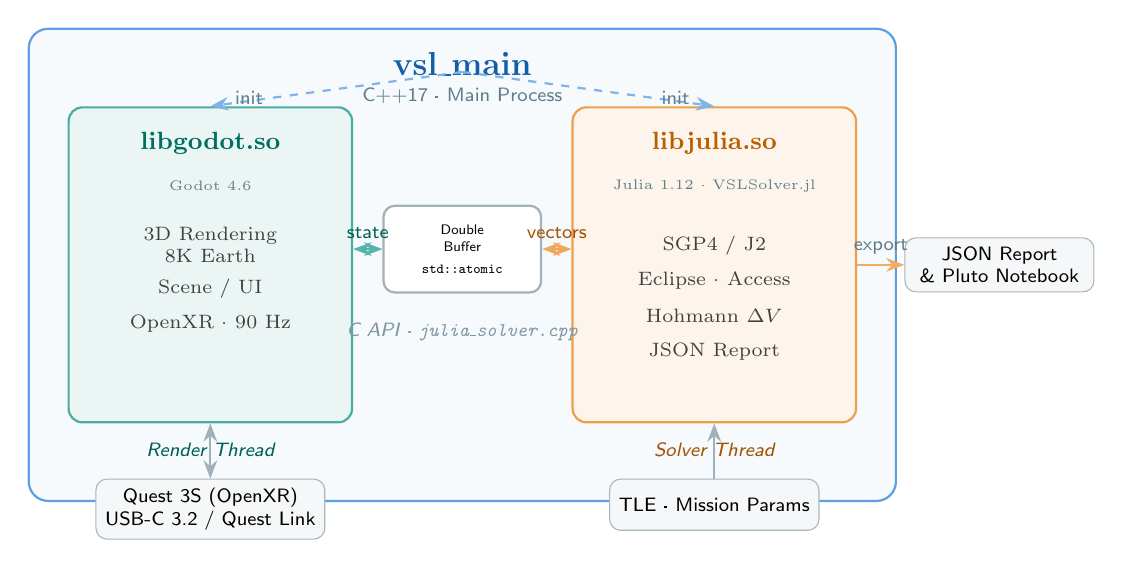
\begin{tikzpicture}[font=\sffamily]

  %% ── Library nodes ──────────────────────────────────────────────────────────

  \node[lib={C1}{}] (godot) at (-3.2, 0) {};
  \node[font=\bfseries\small, text=C1!80!black]        at (-3.2,  1.55) {libgodot.so};
  \node[font=\tiny, text=C3]                            at (-3.2,  1.00) {Godot 4.6};
  \node[font=\scriptsize, text=black!75, align=center]  at (-3.2,  0.25) {3D Rendering\\8K Earth};
  \node[font=\scriptsize, text=black!75]                at (-3.2, -0.30) {Scene / UI};
  \node[font=\scriptsize, text=black!75]                at (-3.2, -0.75) {OpenXR · 90 Hz};

  \node[lib={C2}{}] (julia) at ( 3.2, 0) {};
  \node[font=\bfseries\small, text=C2!80!black]         at ( 3.2,  1.55) {libjulia.so};
  \node[font=\tiny, text=C3]                             at ( 3.2,  1.00) {Julia 1.12 · VSLSolver.jl};
  \node[font=\scriptsize, text=black!75]                 at ( 3.2,  0.25) {SGP4 / J2};
  \node[font=\scriptsize, text=black!75]                 at ( 3.2, -0.20) {Eclipse · Access};
  \node[font=\scriptsize, text=black!75]                 at ( 3.2, -0.65) {Hohmann $\Delta V$};
  \node[font=\scriptsize, text=black!75]                 at ( 3.2, -1.10) {JSON Report};

  %% ── Double buffer ──────────────────────────────────────────────────────────

  \node[buf] (buf) at (0, 0.2) {Double\\Buffer\\[2pt]{\ttfamily\tiny std::atomic}};

  \draw[darr, C1!65]
    (godot.east |- buf.west) -- (buf.west)
    node[midway, above, lbl, text=C1!70!black] {state};

  \draw[darr, C2!65]
    (buf.east) -- (julia.west |- buf.east)
    node[midway, above, lbl, text=C2!70!black] {vectors};

  %% ── Thread labels ──────────────────────────────────────────────────────────

  \node[lbl, text=C1!70!black] at (-3.2, -2.35) {\itshape Render Thread};
  \node[lbl, text=C2!70!black] at ( 3.2, -2.35) {\itshape Solver Thread};

  %% ── C API note ─────────────────────────────────────────────────────────────

  \node[lbl, text=C3!80] at (0, -0.85)
    {\itshape C API · \texttt{julia\_solver.cpp}};

  %% ── vsl_main outer frame ───────────────────────────────────────────────────

  \begin{scope}[on background layer]
    \node[
      rectangle, rounded corners=7pt,
      draw=C0!70, fill=C0!4, thick,
      fit=(godot)(julia)(buf),
      inner xsep=14pt, inner ysep=28pt,
    ] (main) {};
  \end{scope}

  % Header labels inside main
  \node[font=\bfseries\large, text=C0!80!black]
    at (main.north |- {(0, 2.55)}) {vsl\_main};
  \node[lbl] at (main.north |- {(0, 2.15)}) {C++17 · Main Process};

  % Init dashed arrows from header to libs
  \draw[arr, dashed, C0!55]
    (0, 2.45) -- (godot.north)
    node[near end, left, lbl] {init};
  \draw[arr, dashed, C0!55]
    (0, 2.45) -- (julia.north)
    node[near end, right, lbl] {init};

  %% ── External nodes ─────────────────────────────────────────────────────────

  % Quest 3S
  \node[ext, below=0.7cm of godot] (vr)
    {Quest 3S (OpenXR)\\USB-C 3.2 / Quest Link};
  \draw[darr, C3!60] (godot.south) -- (vr.north);

  % TLE input
  \node[ext, below=0.7cm of julia] (tle)
    {TLE · Mission Params};
  \draw[arr, C3!60] (tle.north) -- (julia.south);

  % JSON output
  \node[ext, right=0.6cm of julia] (json)
    {JSON Report\\\& Pluto Notebook};
  \draw[arr, C2!60] (julia.east) -- (json.west)
    node[midway, above, lbl] {export};

\end{tikzpicture}
\end{document}
